% Template:     Informe/Reporte LaTeX
% Documento:    Archivo principal
% Versión:      5.4.7 (25/06/2018)
% Codificación: UTF-8
%
% Autor: Pablo Pizarro R. @ppizarror
%        Facultad de Ciencias Físicas y Matemáticas
%        Universidad de Chile
%        pablo.pizarro@ing.uchile.cl, ppizarror.com
%
% Manual template: [http://latex.ppizarror.com/Template-Informe/]
% Licencia MIT:    [https://opensource.org/licenses/MIT/]

% CREACIÓN DEL DOCUMENTO
\documentclass[letterpaper,11pt]{article} % Articulo tamaño carta, 11pt
\usepackage[utf8]{inputenc} % Codificación UTF-8
\usepackage{subcaption} 

% INFORMACIÓN DEL DOCUMENTO
\def\titulodelinforme {Control Adaptativo}
\def\temaatratar {Ejercicio $N^{o}$ 1}

\def\autordeldocumento {Fran Herrera Rojas}
\def\nombredelcurso {Control Adaptivo de Sistemas}
\def\codigodelcurso {EL-7017}

\def\nombreuniversidad {Universidad de Chile}
\def\nombrefacultad {Facultad de Ciencias Físicas y Matemáticas}
\def\departamentouniversidad {Departamento de la Universidad}
\def\imagendepartamento {departamentos/fcfm}
\def\imagendepartamentoescala {0.2}
\def\localizacionuniversidad {Santiago, Chile}

% INTEGRANTES, PROFESORES Y FECHAS
\def\tablaintegrantes {
\begin{tabular}{ll}
	Alumna:
	& \begin{tabular}[t]{@{}l@{}}
		Francisca Herrera Rojas \\
	\end{tabular} \\
	Profesor:
	& \begin{tabular}[t]{@{}l@{}}
		Manuel Duarte Mermoud
	\end{tabular} \\
	Auxiliares:
	& \begin{tabular}[t]{@{}l@{}}
		Juan Carlos Travieso \\
	\end{tabular} \\
	Ayudantes:
	& \begin{tabular}[t]{@{}l@{}}
	Lisbel Bárzaga\\
	\end{tabular} \\
	\multicolumn{2}{l}{} \\
	& \\
	\multicolumn{2}{l}{Fecha de realización: \today} \\
	\multicolumn{2}{l}{Fecha de entrega: \today} \\
	\multicolumn{2}{l}{\localizacionuniversidad}
\end{tabular}}{
}

% CONFIGURACIONES
\input{lib/config}

% IMPORTACIÓN DE LIBRERÍAS
\input{lib/env/imports}

% IMPORTACIÓN DE FUNCIONES Y ENTORNOS
\input{lib/cmd/all}

% IMPORTACIÓN DE ESTILOS
\input{lib/style/all}

% CONFIGURACIÓN INICIAL DEL DOCUMENTO
\input{lib/cfg/init}

% INICIO DE LAS PÁGINAS
\begin{document}

% PORTADA
\input{lib/page/portrait}

% CONFIGURACIÓN DE PÁGINA Y ENCABEZADOS
\input{lib/cfg/page}

% RESUMEN O ABSTRACT

% TABLA DE CONTENIDOS - ÍNDICE
\input{lib/page/index} % Índice, se puede borrar

% CONFIGURACIONES FINALES
\input{lib/cfg/final}

% ======================= INICIO DEL DOCUMENTO =======================

\section{Problema 1}
Considerando la planta lineal inestable y desconocida de primer orden:
\begin{align}
    \dot{y_{p}}(t)-3y_{p}(t)=2u(t)&&y_{p}(0)=-0.5
\end{align}
y el modelo de referencia lineal asintoticamente estable de primer orden:
\begin{align}
     \dot{y_{m}}(t)+0.5y_{m}(t)=3r(t)&&y_{m}(0)=1
\end{align}

El objetivo de esta sección es diseñar diferentes tipos de controladores que permitan que los estados de la planta y modelo, $y_{p}$ e $y_{m}$ respectivamente, converjan a 0 en el denominado error de control $e_{c}(t)$.
\begin{align}
    e_{c}(t)=\lim_{t\rightarrow\infty}(y_{p}(t)-y_{m}(t))=0
\end{align}

Los diferentes tipos de controladores comparten la misma ley de control dada por:
\begin{align}
    u(t)=\theta(t)x_{p}(t)+k(t)r(t)
\end{align}
Se pueden encontrar 2 enfoques respecto al control adaptativo; en uno los parámetros de la planta son estimados en linea y a partir de estas estimaciones se realizan los ajustes de los parámetros de control, este enfoque se denomina \textbf{indirecto}. Por otro lado, el control directo se caracteriza por 





\subsection{Controlador Directo}
\subsubsection{Leyes de Ajuste }

\subsubsection{Resultados}
En primera instancia se considera una referencia $r(t)$ escalón de amplitud 1 y ganancias adaptativas $sgn(k_{p})=1$ tanto para $\theta(t)$ y $k(t)$, obteniéndose los siguientes resultados para la evolucionó de los estados y la convergencia del error de control.

 \begin{figure}
  \begin{subfigure}[b]{0.4\textwidth}
    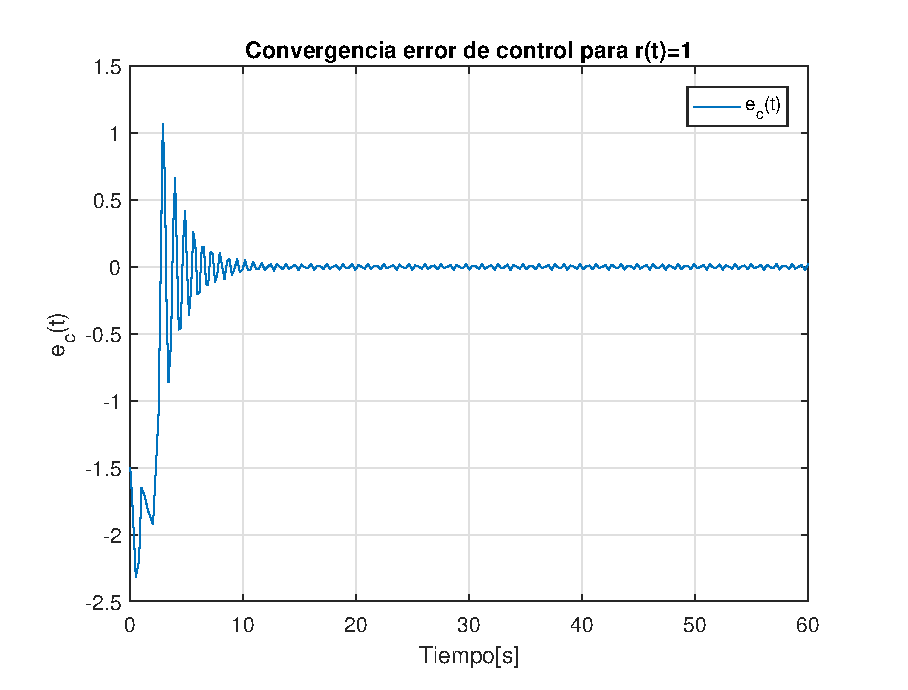
\includegraphics[width=\textwidth]{error_r1.eps}
    \caption{Convergencia error de control para r(t)=1 escalón}
    \label{fig:error_r1}
  \end{subfigure}
  \begin{subfigure}[b]{0.4\textwidth}
    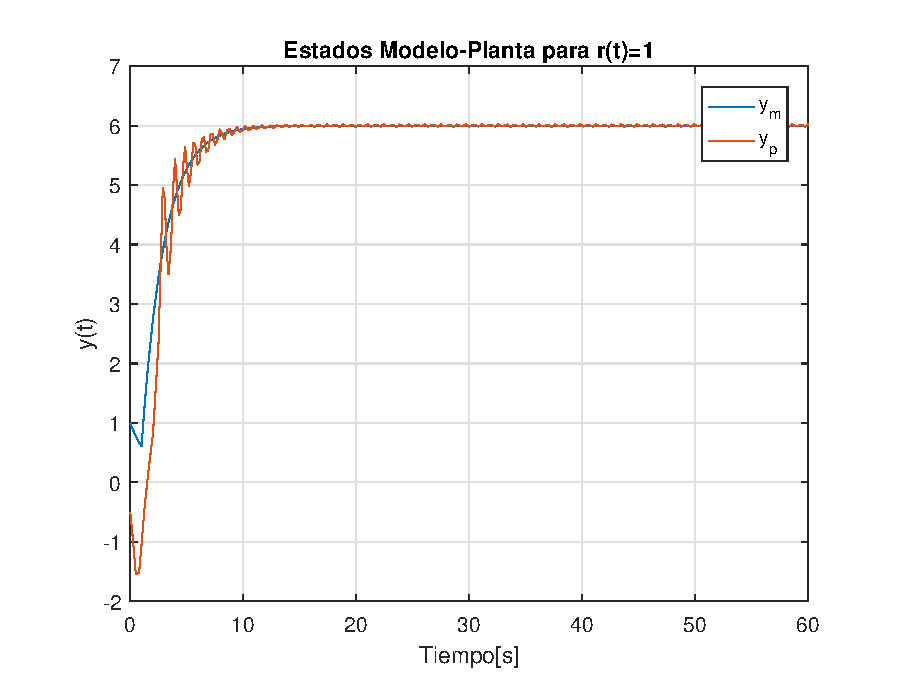
\includegraphics[width=\textwidth]{estados_r1.eps}
    \caption{Estados para r(t)=1 escalón}
    \label{fig:est_r1}
  \end{subfigure}
\end{figure}

 \begin{figure}
  \begin{subfigure}[b]{0.4\textwidth}
    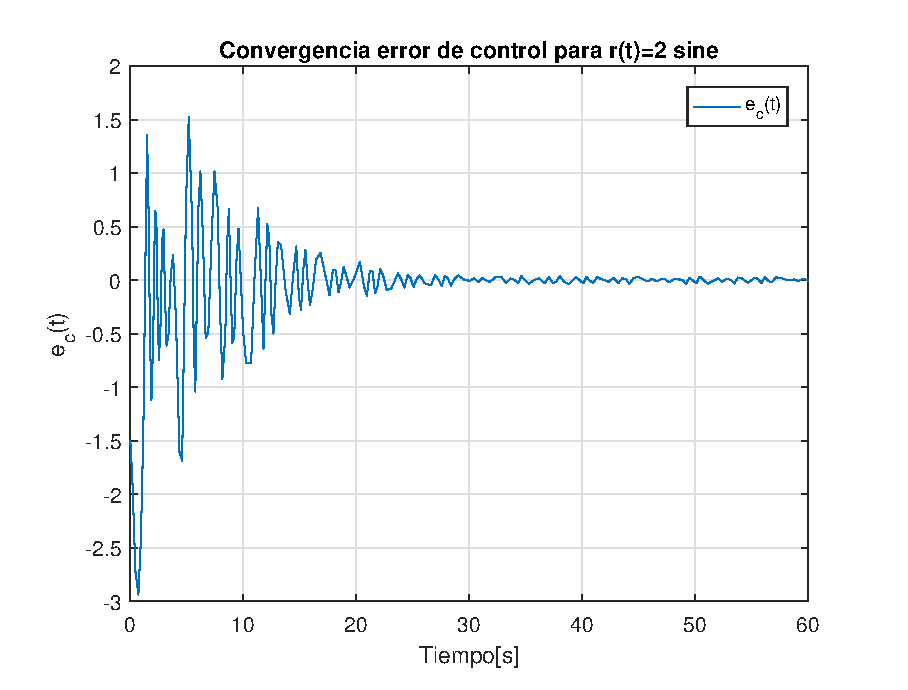
\includegraphics[width=\textwidth]{error_sine2.eps}
    \caption{Convergencia error de control para r(t)=2 sine}
    \label{fig:error_sine2}
  \end{subfigure}
  \begin{subfigure}[b]{0.4\textwidth}
    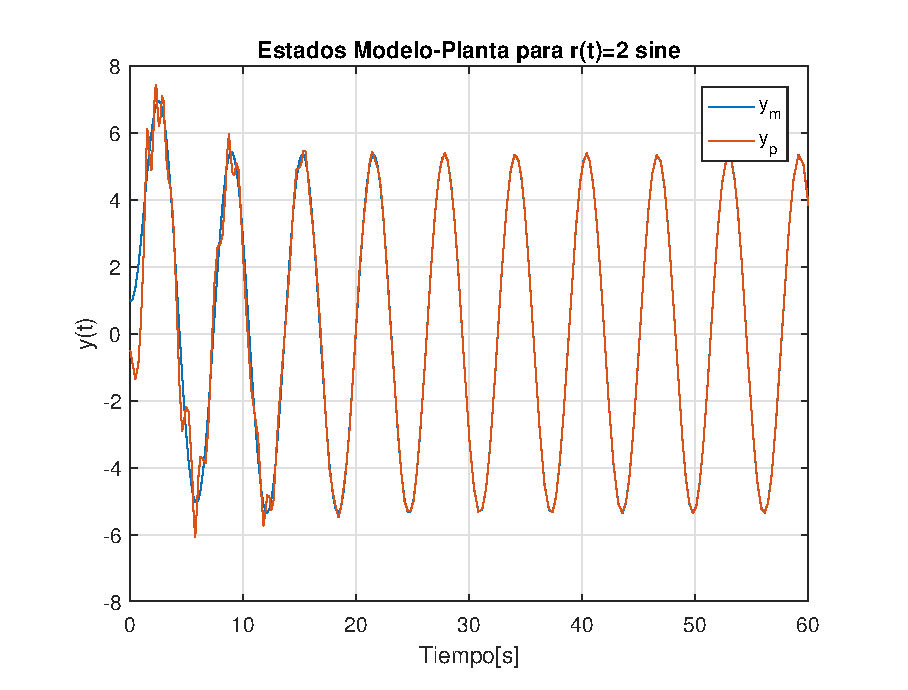
\includegraphics[width=\textwidth]{estados_sine2.eps}
    \caption{Estados para r(t)=2 sine}
    \label{fig:est_sine2}
  \end{subfigure}
\end{figure}

De acuerdo a las Figuras [\ref{fig:error_r1}][ \ref{fig:error_sine2}] es posible apreciar que al iniciar la simulación se presentan oscilaciones propias del comportamiento inestable de la planta; estas oscilaciones son de mayor duración para $r(t)$ sine de amplitud 2. No obstante, en ambos casos se logra la estabilización de la planta.














\subsection{Controlador Indirecto Algebraico}
\subsubsection{Leyes de Ajuste }

\subsubsection{Resultados}


\subsection{Controlador Indirecto Dinámico}
\subsubsection{Leyes de Ajuste }

\subsubsection{Resultados}


\subsection{Controlador Indirecto Combinado}
\subsubsection{Leyes de Ajuste }

\subsubsection{Resultados}




\section{Problema 2}
Considerando el sistema de segundo orden definido por:
\begin{align}
    \dot{x}(t)=\begin{bmatrix}
a_{11} & a_{12}\\ 
 a_{21}& a_{22}x(t)
\end{bmatrix}+\begin{bmatrix}
b_{1}\\ 
b_{2}
\end{bmatrix}u(t)&&
y(t)=\begin{bmatrix}
c_{1}&c_{2}
\end{bmatrix}
\end{align}





\subsection{Observador basado en una realización mínima para el sistema.}

\subsection{Observador basado en una realización no mínima para el sistema.}

Ahora utilizando los siguientes valores para los parámetros:
\begin{align}
    A=\begin{bmatrix}
0&1\\ 
-2&-3
\end{bmatrix}&&b=\begin{bmatrix}
1\\ 
1
\end{bmatrix}&&c=\begin{bmatrix}
0\\ 
1
\end{bmatrix}
\end{align}
\subsection{}

\subsection{}

\subsection{}

 % Ejemplo, se puede borrar

% FIN DEL DOCUMENTO
\end{document}
